\documentclass[tikz, dvipsnames]{standalone}
\usetikzlibrary{matrix,positioning}
\colorlet{rulecolor}{red!15}

% arara: pdflatex: { draft: yes }
% arara: pdflatex: { synctex: no }
% arara: latexmk:  { clean: partial }
\begin{document}
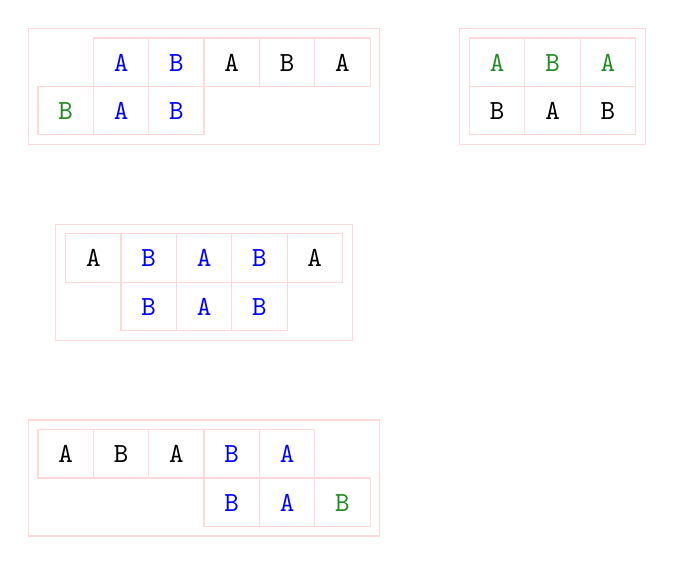
\begin{tikzpicture}[
		,cell/.style = {
			rectangle,
			draw = rulecolor}
		,insert/.style = { text = ForestGreen }
		,ok/.style = { text = blue }
		,space/.style = {
			,matrix of nodes
			,minimum height = 1.5em
			,row sep	= -\pgflinewidth
			,column sep	= -\pgflinewidth
			,column 1/.style = {font = \ttfamily}
		}
		,text depth		= 0.5ex,
		,text height	= 2ex,
		% ,nodes in empty cells
		,font=\ttfamily
		,nodes = {cell, minimum width = 2em}
]

\matrix (first) [space]{
	&|[ok]|A&|[ok]|B&A&B&A \\
	|[insert]|B&|[ok]|A&|[ok]|B&& \\
};

\matrix (second) [space, below = of first]{
	A&|[ok]|B&|[ok]|A&|[ok]|B&A \\
	&|[ok]|B&|[ok]|A&|[ok]|B& \\
};

\matrix (third) [space, below = of second]{
	A&B&A&|[ok]|B&|[ok]|A \\
	&&&|[ok]|B&|[ok]|A&|[insert]|B \\
};

\matrix (ok) [space, right = of first]{
	|[insert]|A & |[insert]|B & |[insert]|A \\
	B&A&B \\
};

\end{tikzpicture}
\end{document}
